\subsection{Electric Potential and Potential Energy} 

%\DTMnewdatestyle{dateupdated}{〈definition 〉

Answers to M\Alph{subsection} problems are on page \pageref{potential_prob_answers}.  \textbf{\textcolor{red}{Updated \DTMnow.}}

%--------------------------------------------------------------------------------------------------------------
\figuretoright{0.30}[scale=0.95]{M_problems/potential/diagonal_force_on_block.pdf}{
\begin{Exercise}
(\textit{Physics 131 Review Problem}) 
A block of mass $m=2.5$~kg is pushed a distance $d=2.2$~m along
a frictionless, horizontal table by a constant applied force of magnitude $F=16$~N, 
directed at $\theta=25 \deg$ below the horizontal, as shown.  
Determine (a)~the work done on the block by the applied force, (b)~the work done by the normal force exerted by the table, 
(c)~the work done by the gravitational force, and (d)~the net work done on the block.  
\end{Exercise}
\begin{Answer}
Two of them are 31.9 Joules, and two of them are zero.
\end{Answer}
}

%--------------------------------------------------------------------------------------------------------------
\figuretoright{0.30}[scale=0.95]{M_problems/potential/work_for_three_paths.pdf}{
\begin{Exercise}
(\textit{Physics 131 Review Problem}) A constant force $\vec{F} = (3\hat{i}+4\hat{j})$~N acts on an object. 
The force does not vary with time or with the position or velocity of the object.  
Using the general definition for work done by a force \(\displaystyle W = \int_\text{i}^\text{f} \vec{F} \cdot d\vec{s}\), 
calculate directly the work done by $\vec{F}$ on the particle as it moves from the origin $O$ to point $C$ along each of the three paths shown.  
\end{Exercise}
\begin{Answer}
At least one of them is 35 Joules.
\end{Answer}


%--------------------------------------------------------------------------------------------------------------
\begin{Exercise}
(a) Find the electric potential a distance 1.0~cm away from a proton.  
(b)~What is the potential difference between two points that are 1.0~cm and 2.0~cm from a proton?  
(c)~Repeat parts (a) and (b) for an electron.  
\end{Exercise}
\begin{Answer}
(a) $+144$ nV (b) $-72$ nV (c) $-144$ nV, $+72$ nV
\end{Answer}
}


%--------------------------------------------------------------------------------------------------------------
\figuretoright{0.46}[scale=0.94]{M_problems/potential/quarter_circle_ramp.pdf}{
\begin{Exercise}
A small block is released from rest at the top of a frictionless, quarter-circle ramp of radius $R$.  The block has a mass $m$ and a charge $q$, and is subject to a uniform external field $\vec{E}$ directed horizontally to the right.  What is the speed of the particle when it reaches the bottom of the ramp?
\end{Exercise}
\begin{Answer}
$v_\text{f} = \sqrt{2R(g-qE/m)}$. 
(Hint: start by drawing some equipotential lines on the figure.)
\end{Answer}


%--------------------------------------------------------------------------------------------------------------
\begin{Exercise}
Two particles with charge $2.0~\mu$C are placed at $x=+0.8$~m and $x=-0.8$~m.  
A small ``test charge'' with $q=1.28 \times 10^{-18}$~C is placed at the origin.  
Find (a)~the electric field at the origin due to the two $2~\mu$C  charges, 
(b)~the force on the test charge, and 
(c)~the electric potential at the origin due to the two $2~\mu$C charges. 
\end{Exercise}
\begin{Answer}
One of the three answers begins with the digits ``449''.  The other two answers are zero.
\end{Answer}
}
\begin{center}
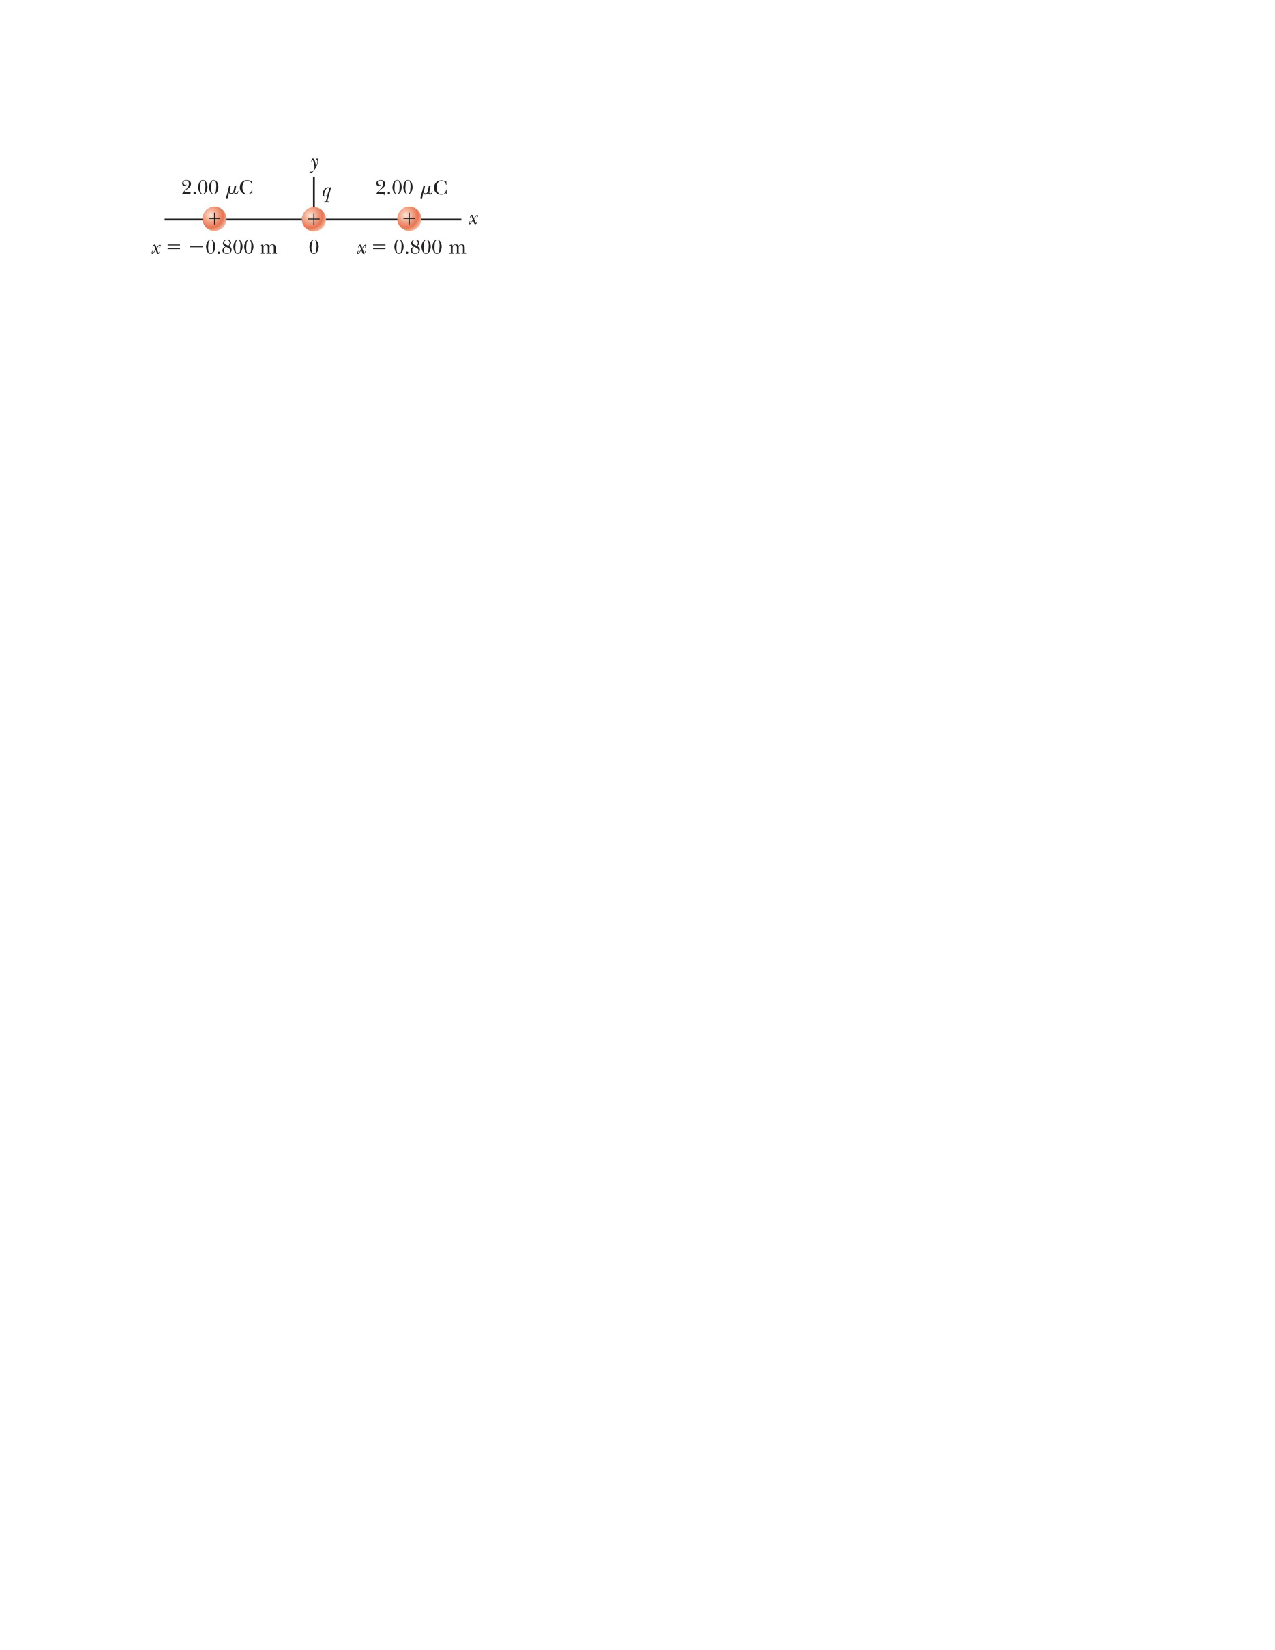
\includegraphics[scale=0.95]{M_problems/potential/three_charges.pdf}
\end{center}



%--------------------------------------------------------------------------------------------------------------
\begin{Exercise}
A $+4$~nC charge is at the origin, and a $+7$~nC charge is at the point $(0, -4\text{ m})$. 
(a)~Find the electric field at the point $(3\text{ m}, 0)$.  
(b)~Find the electric potential at $(3\text{ m}, 0)$.  
(c)~Which part was easier, part (a) or part (b), and why?
\end{Exercise}
\begin{Answer}
(a) $(5.51 \hat{i} + 2.01 \hat{j})$~N/C (b) 24.6 volts
\end{Answer}


%--------------------------------------------------------------------------------------------------------------
\begin{Exercise}
Three charged particles lie along the $x$ axis: a charge $+Q$ is at $x=0$, and two charges $-Q$ are at $x=\pm a$.  (a)~Draw a graph of potential $V$ as a function of $x$ along the axis.  
(b)~Draw a graph of electric field $E$ as a function of $x$ along the axis, where the sign of the field indicates its direction.  
(c)~At $x=\pm a/2$ is $V$ positive, negative, or zero?  
(d)~At $x=\pm a/2$ is $E$ positive, negative, or zero?  Explain your reasoning for parts (c) and (d). 
\begin{center}
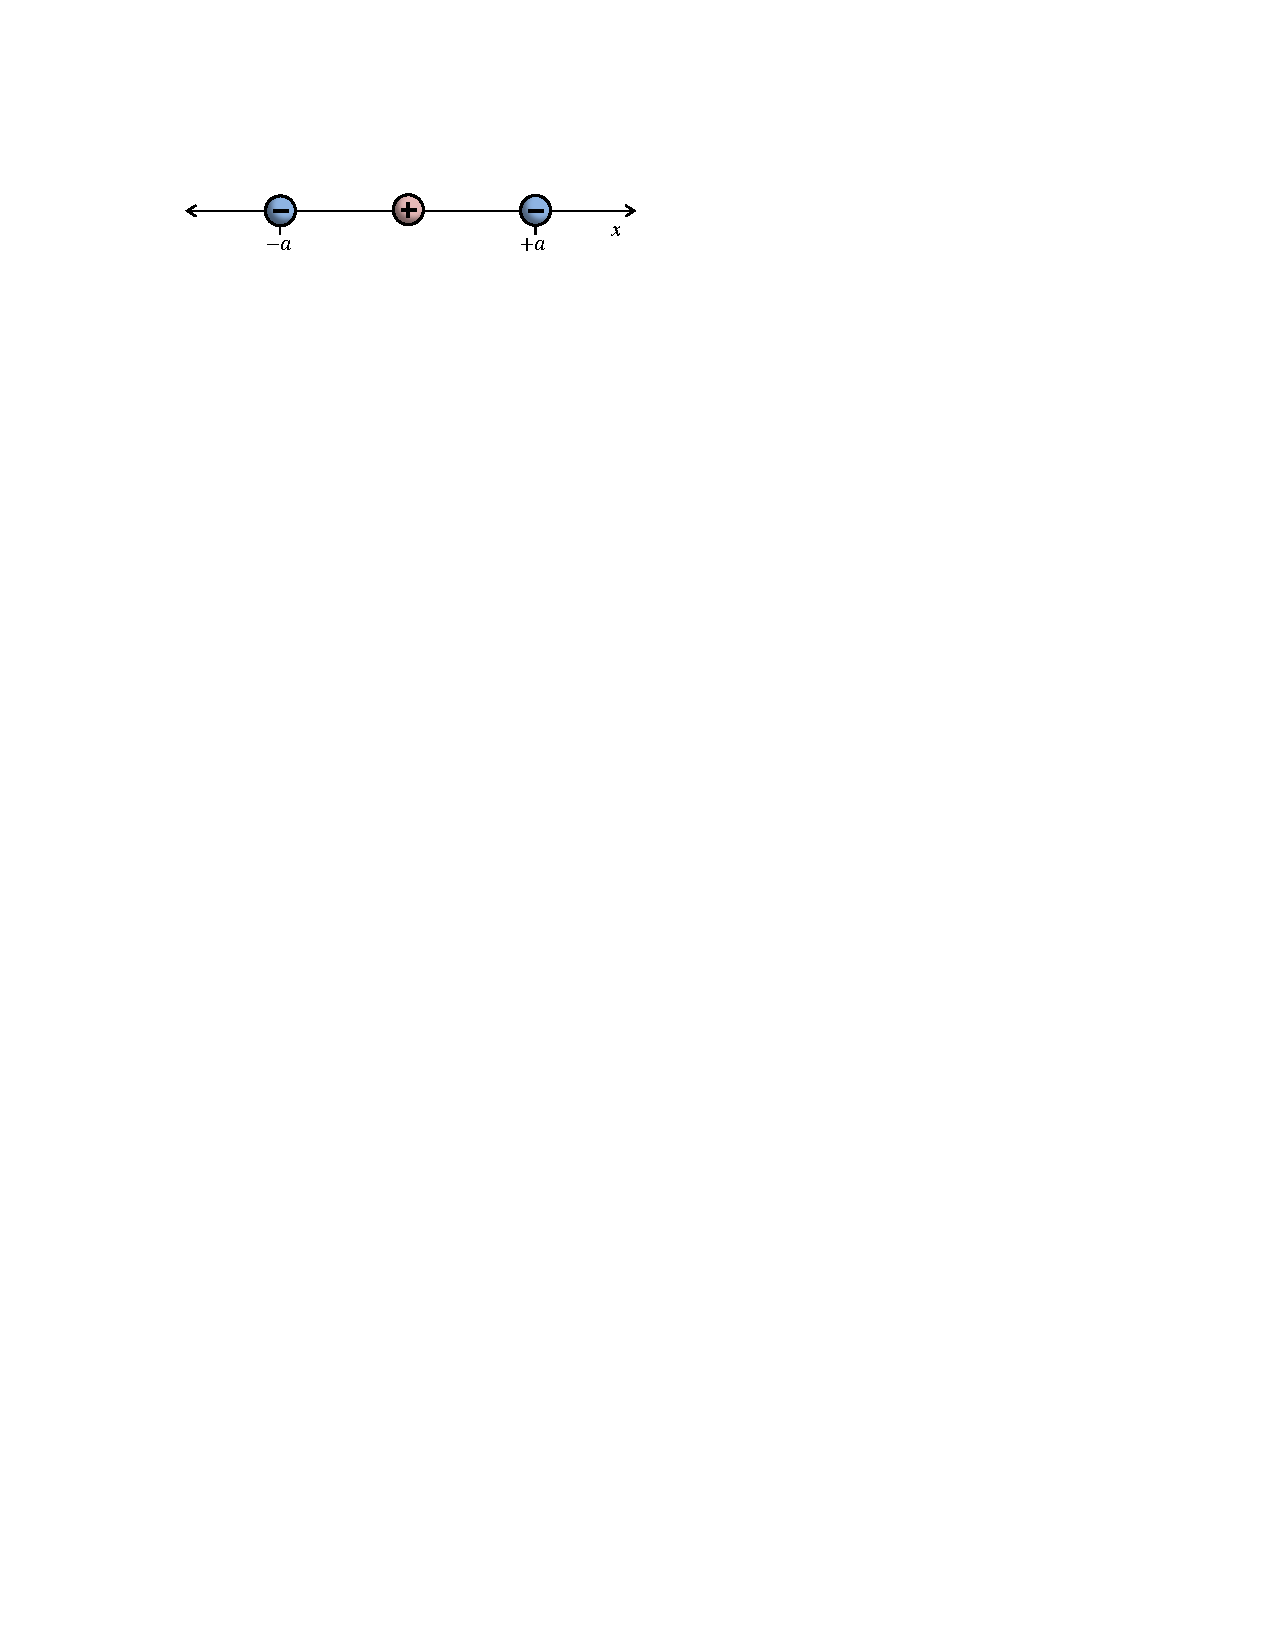
\includegraphics{M_problems/potential/quadrupole.pdf}
\end{center}

\end{Exercise}
\begin{Answer}
(c) $V \left( -\frac{a}{2} \right) =V \left( -\frac{a}{2} \right) < 0$ (d) $E \left( -\frac{a}{2} \right) <0, E \left( +\frac{a}{2} \right)>0$
\end{Answer}

%--------------------------------------------------------------------------------------------------------------
\begin{Exercise}
A $+5$~nC charge sits on the $y$ axis at (0, 3~cm), and a $-2$~nC charge sits at (3~cm, 3~cm) as shown.  
(a)~Find the potential $V$ at the points $P_1$ and $P_2$ shown.  
(b)~What is the change in potential energy $\Delta U$ of the system when a third particle, of charge $q_3=+3$~nC and mass $m=4~\mu\text{g} (4 \times 10^{-9}~\text{kg})$, is brought in from very far away to position $P_1$?  
(c)~How much work is required to move the $+3$~nC particle from point $P_1$ to point $P_2$?  
(d) The $+3$~nC particle is released from position $P_2$, and it accelerates away from both other charges.  What is the maximum velocity attained by the charge once it is very far away?
\begin{center}
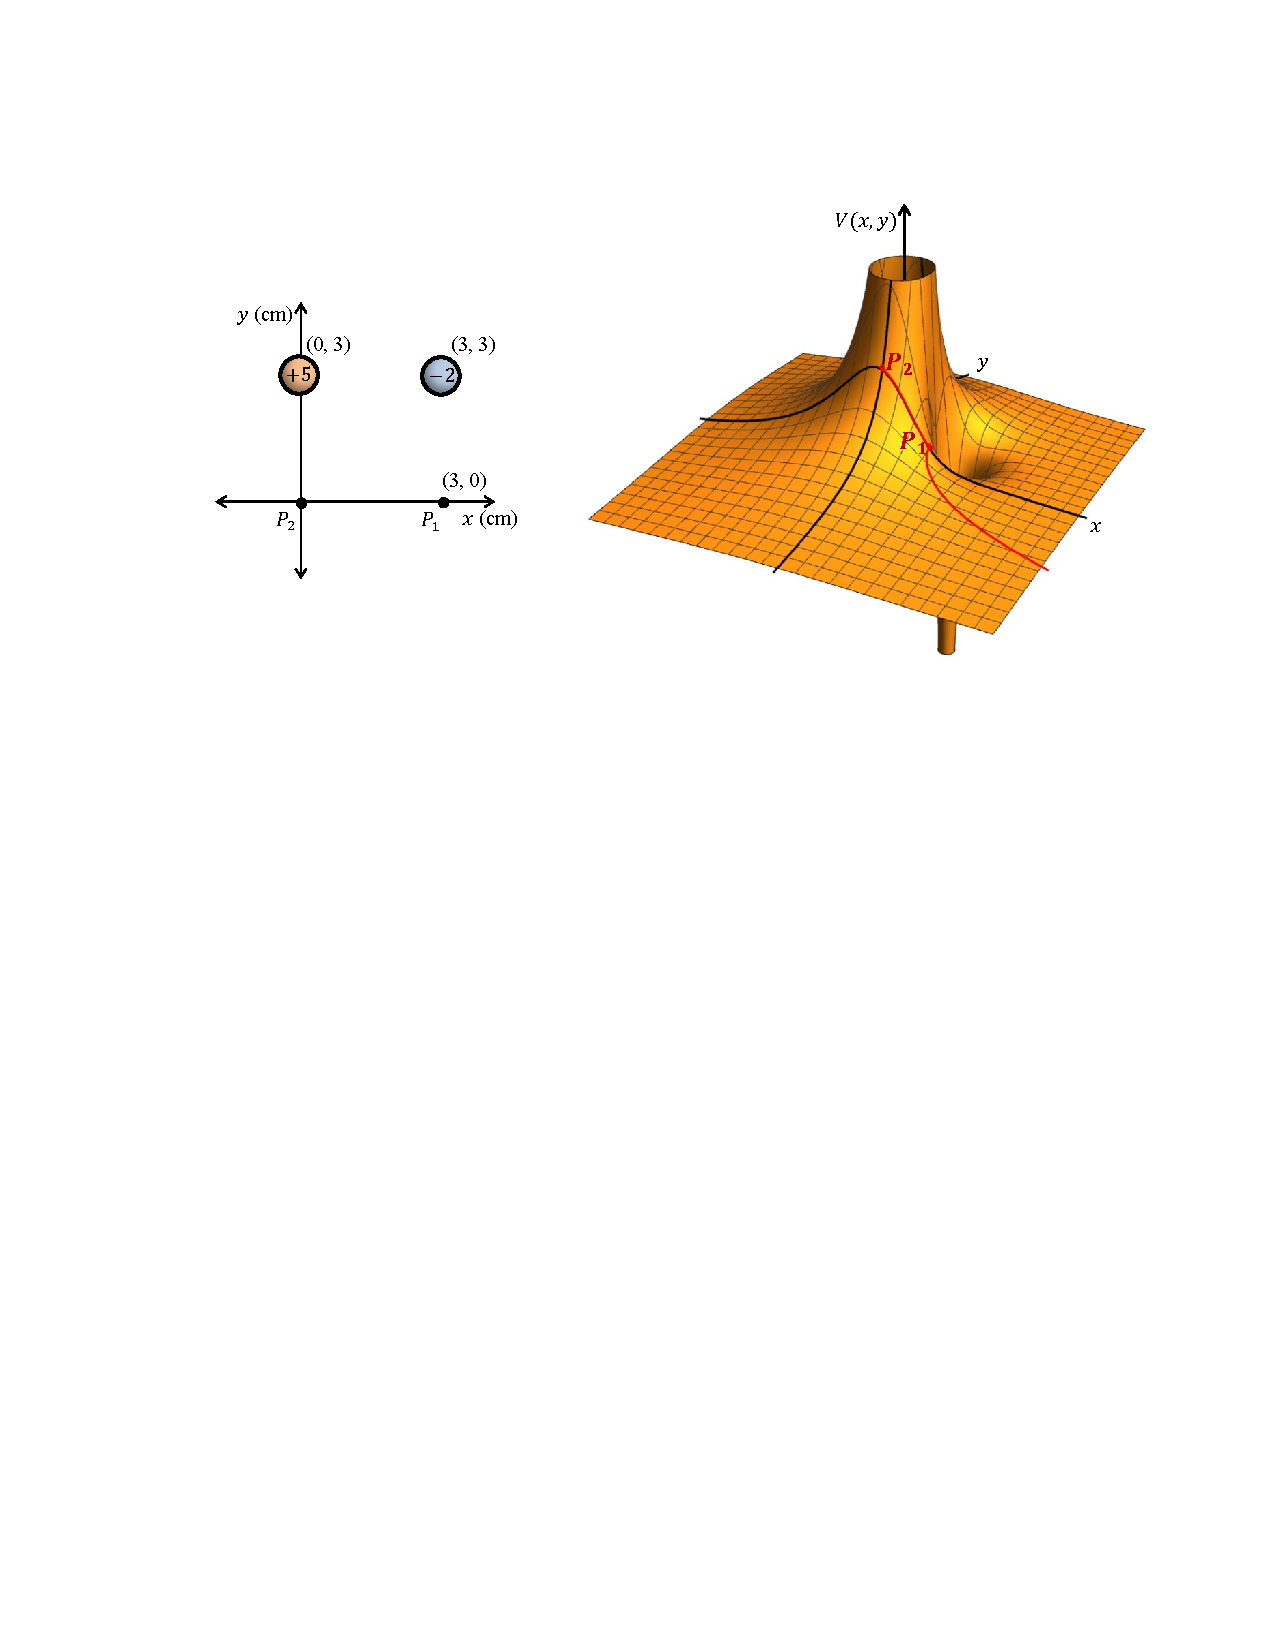
\includegraphics{M_problems/potential/potential_surface.pdf}
\end{center}

\end{Exercise}
\begin{Answer}
(a) 460 V and 1075 V (b) $1.38~\mu$J  (c) $1.84~\mu$J  (d) 40.2 m/s
\end{Answer}

%--------------------------------------------------------------------------------------------------------------
\figuretoright{0.25}[scale=0.95]{M_problems/potential/four_charges.pdf}{
\begin{Exercise}
Four identical particles, all with $q=+10~\mu$C are located on the corners of a rectangle ($L=0.6$~m, $W=0.15$~m) as shown.  
Calculate the change in electric potential energy of the system as the particle at the lower left corner of the figure is brought to this position from infinitely far away.
(The other three particles remain fixed in position during the process.) 
\end{Exercise}
\begin{Answer}
8.94 J
\end{Answer}
}

%--------------------------------------------------------------------------------------------------------------
\begin{Exercise}
A thin rod of length $L=20$~cm, with a total positive charge $Q=10$~nC, lies on the $y$ axis between $y=0$ and $y=20$~cm.  
In this problem, you will calculate the electric potential $V$ at a point along the $x$ axis a distance $x=15$~cm from the origin.  
(a)~First, estimate it numerically, using a spreadsheet program like Excel.  
Divide the rod into ten individual 1~nC charges located at $y=1$~cm, $y=3$~cm, etc., up to $y=19$~cm.  
Treat each as a point charge, and find the potential at the point $x=15$~cm, $y=0$ due to all of them.  
(b)~Now solve the problem exactly by setting up and solving an integral over the entire length of the rod.  
\end{Exercise}
\begin{Answer}
(using $k_e=8.99000\times10^9$~Nm$^2/$C$^2$) (a) 493.922 Volts (b) 493.826 Volts
\end{Answer}

%--------------------------------------------------------------------------------------------------------------
\figuretoright{0.35}[scale=0.95]{M_problems/potential/nonuniform_rod.pdf}{
\begin{Exercise}
A rod of length $L$ lies along the $x$ axis with its left end at the origin, as shown in the figure to the right.  
The rod has a nonuniform charge density $\lambda=\alpha x$, where $\alpha$ is a positive constant.  
(That is, the charge density increases linearly over the rod from left to right.)  
(a)~What would be the standard SI units of $\alpha$?  (b)~Calculate the electric potential at point $A$ in the figure.
\end{Exercise}
\begin{Answer}
(a) C/m$^2$ (b): $\displaystyle V=k_e \alpha \left[ L - d \ln \left(1+\frac{L}{d} \right) \right]$
\end{Answer}

%--------------------------------------------------------------------------------------------------------------
\begin{Exercise}
For the arrangement described in the previous problem and pictured to the right, find the electric potential at point $B$, which lies on the perpendicular bisector of the rod a distance $b$ above the axis.  
(For this problem, you can leave your answer in the form of an integral.)
\end{Exercise}
\begin{Answer}
The integral you get is
$\displaystyle \int_0^L \frac{k_e \alpha x}{\sqrt{(x-L/2)^2 +b^2}}dx$,
and as I said in the problem, it's fine with me if you leave it that way. 
\end{Answer}
}

%--------------------------------------------------------------------------------------------------------------
\begin{Exercise}
Suppose the potential energy of a system in which a two-dimensional force acts on an object is given by $U(x,y)=3x^3y-7x$.  
(a)~Find the $x$ component $F_x$ of the force that acts at the point $(x,y)$.  
Hint: you already know that in one dimension along the $x$ axis, the force is related to potential energy by $F = - dU/dx$. The extra ``$y$'' doesn't really change anything. 
(b)~Reasoning by analogy,\footnote{That is, using the advanced mathematical procedure of ``doing it for $y$ instead of $x$.''}
write the $y$ component $F_y$ of the force as well.
(c)~What is the force $\vec{F}$ on the object, written in component form in terms of $\hat{i}\text{~and~}\hat{j}$?
\end{Exercise}
\begin{Answer}
(a) $F_x = -9x^2y +7$ (all you did here was to treat $y$ is a constant; that is, you took a partial derivative, which means that you can look very fancy by writing it as 
$\partial U/\partial x$)
(c) $\vec{F}= (-9x^2 y+7)\hat{i} +(-3x^3)\hat{j}$
\end{Answer}


%--------------------------------------------------------------------------------------------------------------
\begin{Exercise}
In some region of space, the electric potential is given by $V=5x-3x^2 y+2yz^2$, where the coordinates $x, y,$ and $z$ are in meters and $V$ is in volts.\footnote{The units have been left off of the numbers 5, 3, and 2 for visual clarity.}  
(a)~Write expressions for the $x, y,$ and $z$ components of the electric field.  (b)~What is the magnitude of the field at the point $(x=1,y=0,z=-2)$?  
\end{Exercise}
\begin{Answer}
(b) 7.07 N/C
\end{Answer}

%--------------------------------------------------------------------------------------------------------------
\figuretoright{0.15}[scale=0.95]{M_problems/potential/semicircle_rod.pdf}{
\begin{Exercise}
An insulating rod, 14~cm long, carrying a uniform charge of $-7.50~\mu$C is bent into a semicircle.  Find the electric potential at point $O$, the center of the semicircle. 
\end{Exercise}
\begin{Answer}
$-1.51$~MV
\end{Answer}


%--------------------------------------------------------------------------------------------------------------
\begin{Exercise}
\label{easy_integration_review_prob}
A particle maintains a constant velocity of 5~m/s.  
\begin{enumerate}[label=(\alph*), nosep, topsep=-2ex, after={\vspace{2ex}}]
\item What is the change in the particle's postion $\Delta x$ between the times $t=10$~s and $t=30$~s?  
\item Draw a graph of $v$ vs. $t$.  
\item Draw several different possible graphs of position $x$ vs. $t$.  (The particle could start at several different initial positions, after all.)  
\item Write a general function for $x$ as a function of $t$.  Don't forget the integration constant!  
\item Write a general expression for the displacement $\Delta x$, as a definite integral of $v(t)$.  
\item Evaluate your integral in the previous part, writing $\Delta x$ in terms of $v$ and $\Delta t$.  
\item Do you need an integration constant to find $\Delta x$ between, say, $t=10$~s and $t=30$~s?
\end{enumerate}
\end{Exercise}
\begin{Answer}
(a) 100 m (c) Your graphs should have the same slope, but different intercepts.
(d)~$x=\int{v\,dt}=vt+C=vt+x_\text{i}$
(e)~$\Delta x=  \int_{t_\text{i}}^{t_\text{f}}{ v\, dt}$
(f)~$ \Delta x=   \int_{t_\text{i}}^{t_\text{f}}{ v\, dt} = v(t_\text{f} - t_\text{i})=v\Delta t$
(g)~no integration constant required.
\end{Answer}
}

%--------------------------------------------------------------------------------------------------------------
\begin{Exercise}
(This is a companion problem to \ref{easy_integration_review_prob}.) 
A uniform electric field is given by $\vec{E} = 500\hat{i}$~V/m. 
\begin{enumerate}[label=(\alph*), nosep, topsep=-2ex, after={\vspace{2ex}}]
\item What is the change in electric potential $\Delta V$ between the points $x=10$~cm and $x=30$~cm? 
\item Draw a graph of $E$ vs. $x$.
\item Draw several different possible graphs of potential $V$ vs. $x$. (There is no reference voltage defined, after all.)
\item Write a general function for $V$ as a function of $x$.  Don't forget the integration constant! 
\item Write a general expression for $\Delta V$, as a definite integral of $E(x)$.
\item Evaluate your integral in the previous part, writing $\Delta V$ in terms of E and $\Delta x$.
\item Do you need an integration constant to find $\Delta V$ between, say, $x=10$~cm and $x=30$~cm?  
\end{enumerate}
\end{Exercise}
\begin{Answer}
(a) 100 V (c) Your graphs should have the same slope, but different intercepts.
(d)~$V=-\int{E\,dx}=-Ex+C$
(e)~$\Delta V=  -\int_{x_1}^{x_2}{ E\, dx}$
(f)~$ \Delta V=   -\int_{x_1}^{x_2}{ E\, dx} = -E\Delta x$
(g)~no integration constant required.
\end{Answer}

%--------------------------------------------------------------------------------------------------------------
\begin{Exercise}
A conducting metal sphere has a radius of $R$ and carries a positive charge $Q$.  
(a)~Draw a graph of the electric field $E(r)$ covering both inside and outside the sphere.  
(b)~Draw a graph of the electric potential $V(r)$ both inside and outside the sphere.  
(c)~What is the value of the electric potential at the center of the sphere, assuming the usual reference point that $V=0$ at $r \to \infty$? 
(d)~What can you say that is always true about the graph of electric potential inside a conductor?  Hint: See workbook problem 26.7.
\end{Exercise}
\begin{Answer}
(a) Remember, $E=0$ inside a conductor.  (c) $V=k_e Q/R$
\end{Answer}

%--------------------------------------------------------------------------------------------------------------
\begin{Exercise}
For the graph of electric field $E(x)$ to the right, \\
\begin{minipage}{0.55 \textwidth}
(a)~sketch a graph of the potential $V(x)$, 
where the reference is $V(\infty)=0$. (b)~Also using $V(\infty)=0$, write an equation for the potential $V(x)$. It'll be different for $x<2$ and $x>2$, so you'll need to use a curly brace (``\}'') to separate the cases.  (Be careful with your signs and the constants....)  

\vspace*{0.6in}
\end{minipage}
\begin{minipage}{0.44 \textwidth}
\vspace{-0.2in}
\hspace{0.2in}
\begin{lab_axis}[lab_grid,
	scale only axis = true,
	ylabel = {Field $E$ (N/C)},
	xlabel = {$x$ (m)},
	width={2.2in}, height={1.1in},
	xmin=0, xmax=6,
	ymin=0, ymax=7,
	ytick distance = 2,
	xtick distance = 1,
]
\addplot coordinates {(0,0) (2,5) (5,5) (5,0) (6,0)};
\end{lab_axis}
\end{minipage}
\end{Exercise}
\begin{Answer}
$\displaystyle V(x) = \begin{cases}
(-1.25~\text{V/m}^2)x^2 + 20\text{ V}, & \text{if } 0 < x < 2 \\
(-5~\text{V/m})x + 25\text{ V}, &  \text{if } 2 < x < 5 \\
0, &  \text{if } x > 5
\end{cases}$
\end{Answer}


\vspace{0.7in}

\textbf{Answers to Selected {\thesubsection} Problems:}
\label{potential_prob_answers}
%\shipoutExercise
\shipoutAnswer

\cleardoublepage
